\documentclass{article}
\usepackage[utf8]{inputenc}
\usepackage[T1]{fontenc}
\usepackage{graphicx}
\usepackage{hyperref}
\usepackage{geometry}
\geometry{margin=1in}

\title{HUGHILY}
\date{Encyclopaedia Britannica (1771)}

\begin{document}
\maketitle

\section*{Historical source}
\textbf{Entry ID:} \texttt{entry-hughily-1327} \\
\textbf{Volume ID:} 149981670 \\
\textbf{Character Count:} 757

\subsection*{Extracted Text}
HUGHILY, a town of Afai, in the kingdom of
Bangels, feated on the molt velocity branch of the in-
ver changes. It is of large extent, reaching about
two miles along the river, flat, and dress a great trade
all all the commodities of this country, affirming cik
cargos for 50 to Ohio annually, besides what is
though to cartages so the neighboring towns,
Solitpere is brought hitner from Patnia in refels above
50 yards long and five broad. The inhabitants are
chely linking but there are also Deutsche Forge,
ilib, and other Europens. E. Long. 87, 55. N.
Las 24.0.

HUGO CAvery, chief of the third race of the kings
of France, being count of Parra and Orleans; he was
refiled to the chrome for his military vollor and public
resturs in 287. See Fears, n 38.



\section*{Source record}
\begin{itemize}
\item \textbf{Dataset:} \texttt{NationalLibraryOfScotland/encyclopaedia\_britannica\_illustrated}
\item \textbf{Dataset Revision:} \texttt{309f765b1ecc83e0a7f7762e44b4a927a7555443}
\item \textbf{Page ID:} \texttt{britannica:309f765b1ecc83e0a7f7762e44b4a927a7555443:train:1327} \\
  \textbf{Filename:} \texttt{page-1327-7d41b1db21d5.jpg} \\
  \textbf{Row Index:} 1327 \\
  \textbf{SHA256:} \texttt{7d41b1db21d5e291...}
\end{itemize}

\begin{figure}[h]
\centering
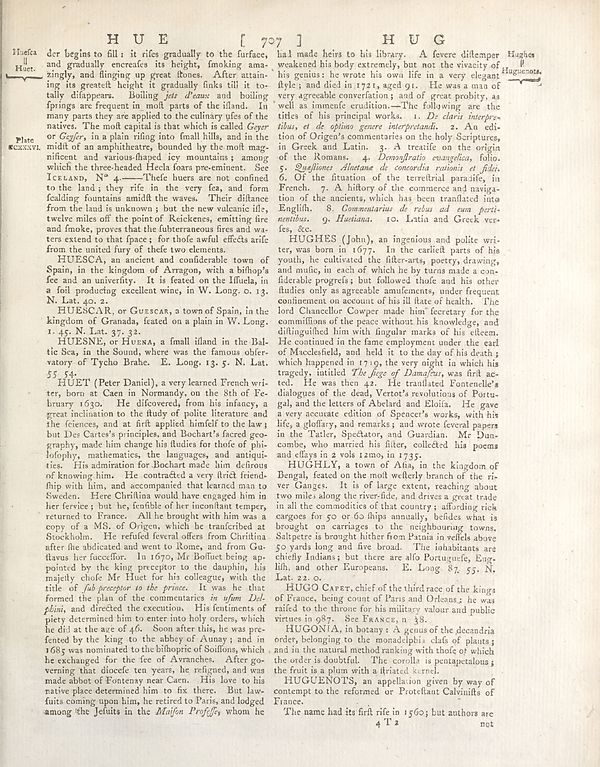
\includegraphics[width=0.85\textwidth]{../scans/page-1327-7d41b1db21d5.jpg}
\caption*{Source scan: \texttt{page-1327-7d41b1db21d5.jpg}}
\end{figure}

\end{document}
